\documentclass[12pt]{article}

\usepackage{mathtools}
\usepackage{amssymb}
\usepackage{atbegshi}% http://ctan.org/pkg/atbegshi
\usepackage{graphicx}
\usepackage{physics}
\AtBeginDocument{\AtBeginShipoutNext{\AtBeginShipoutDiscard}}

\usepackage{fontspec}
\defaultfontfeatures{Mapping=tex-text,Scale=MatchLowercase}
\setmonofont{Consolas}


\begin{document}

\title{Tarea 25\\
	\large Elementos de ciencias de la computación}

\author{Tulio Muñoz Magaña}
\today
\maketitle

\textbf{Inciso b)}\\

El programa sirve para copiar todo el contenido de un archivo de texto a otro, solo que propone dos alternativas diferentes para leer caracteres (\texttt{fscanf} y \texttt{getc}) y dos para colocarlos en el nuevo archivo (\texttt{fprintf} y \texttt{putc}).\\

Funcionan ligeramente diferente las funciones \texttt{fscanf} y \texttt{getc}, la primera recibe como parámetro la dirección de la variable donde se va a guardar el caracter que se está leyendo, además de que se tiene que especificar que se leerá un caracter. La función regresa el número de datos correctamente leidos y asignados, regresa $-1$ si el archivo se ha terminado.\\
La función \texttt{getc} por otro lado, es específica para caracteres, por lo que no se tiene que especificar que se leerá un caracter, recibe como parámetro solamente el archivo y regresa por la izquierda el caracter leido.\\

El programa imprime en consola los caracteres que va copiando, seguidos de su valor en ASCII. \\
La diferencia entre el uso de \texttt{fscanf} y \texttt{getc} en el código es que cuando se usa \texttt{fscanf} el programa se sale del ciclo cuando la función regresa $-1$ y se imprime en consola este valor junto con el valor del último caracter copiado.\\
Cuando se utiliza \texttt{getc} se imprime \texttt{EOF} cuando la función \texttt{getc} arroja este valor y se sale del ciclo.\\

En ambos casos al finalizar se imprime \texttt{FIN DE CICLO}.\\

La diferencia más notoria entre \texttt{fprintf} y \texttt{putc} es que en la primer se tiene que especificar que se va a escribir un caracter, y en la segunda no porque está escrita especialmente para eso.\\

\textbf{Punto opcional.}\\

A continuación vemos lo que el editor hexadecimal muestra con los distintos archivos de la tarea.\\

\texttt{sample.txt}\\

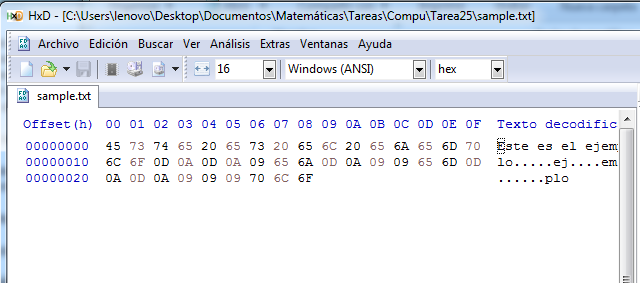
\includegraphics[width = \textwidth]{sam}\\

\texttt{result.txt}\\

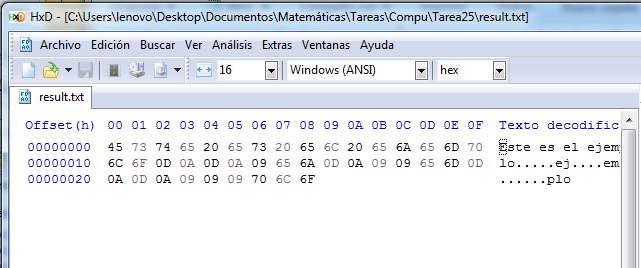
\includegraphics[width = \textwidth]{res}\\

\texttt{map.txt}\\

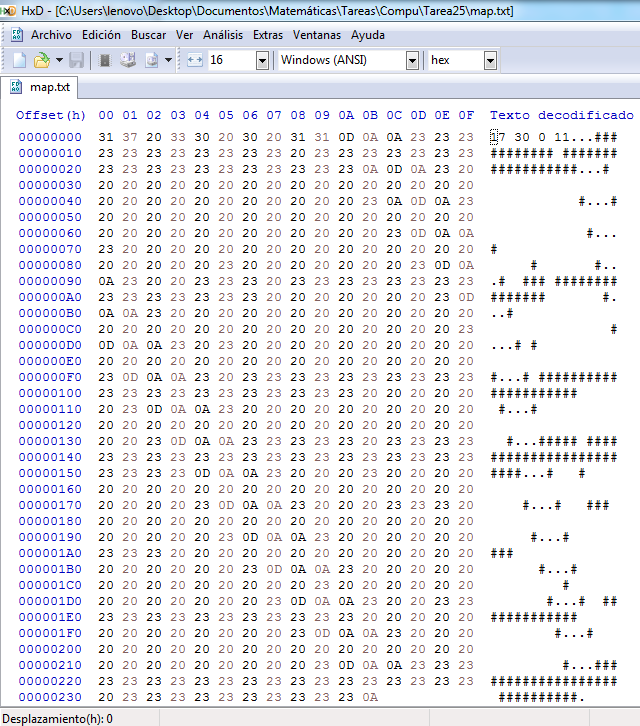
\includegraphics[width = \textwidth]{m}\\

En efecto se muestra lo esperado.\\
























\end{document}